\section{Bài 2: HTTP}
Xóa cache browser trước khi truy cập trang web hoặc dùng ẩn danh. Dùng Wireshark để bắt gói tin khi truy cập vào website: http://example.com.\\
Việc bắt gói tin bằng Wireshark trong bài được thực hiện bằng \textbf{máy ảo}, sử dụng hệ điều hành \textbf{Windows Server 2012 R2}.\\
Kết quả bắt gói tin chi tiết được lưu trong tập tin \textbf{\textit{bai2.pcapng}}.

\textbf{1. Chụp hình kết quả bắt gói tin từ lúc bắt đầu DNS đến lúc gửi HTTP request (thấy được những gói tin liên quan).}
\begin{figure}[H]
\begin{center}
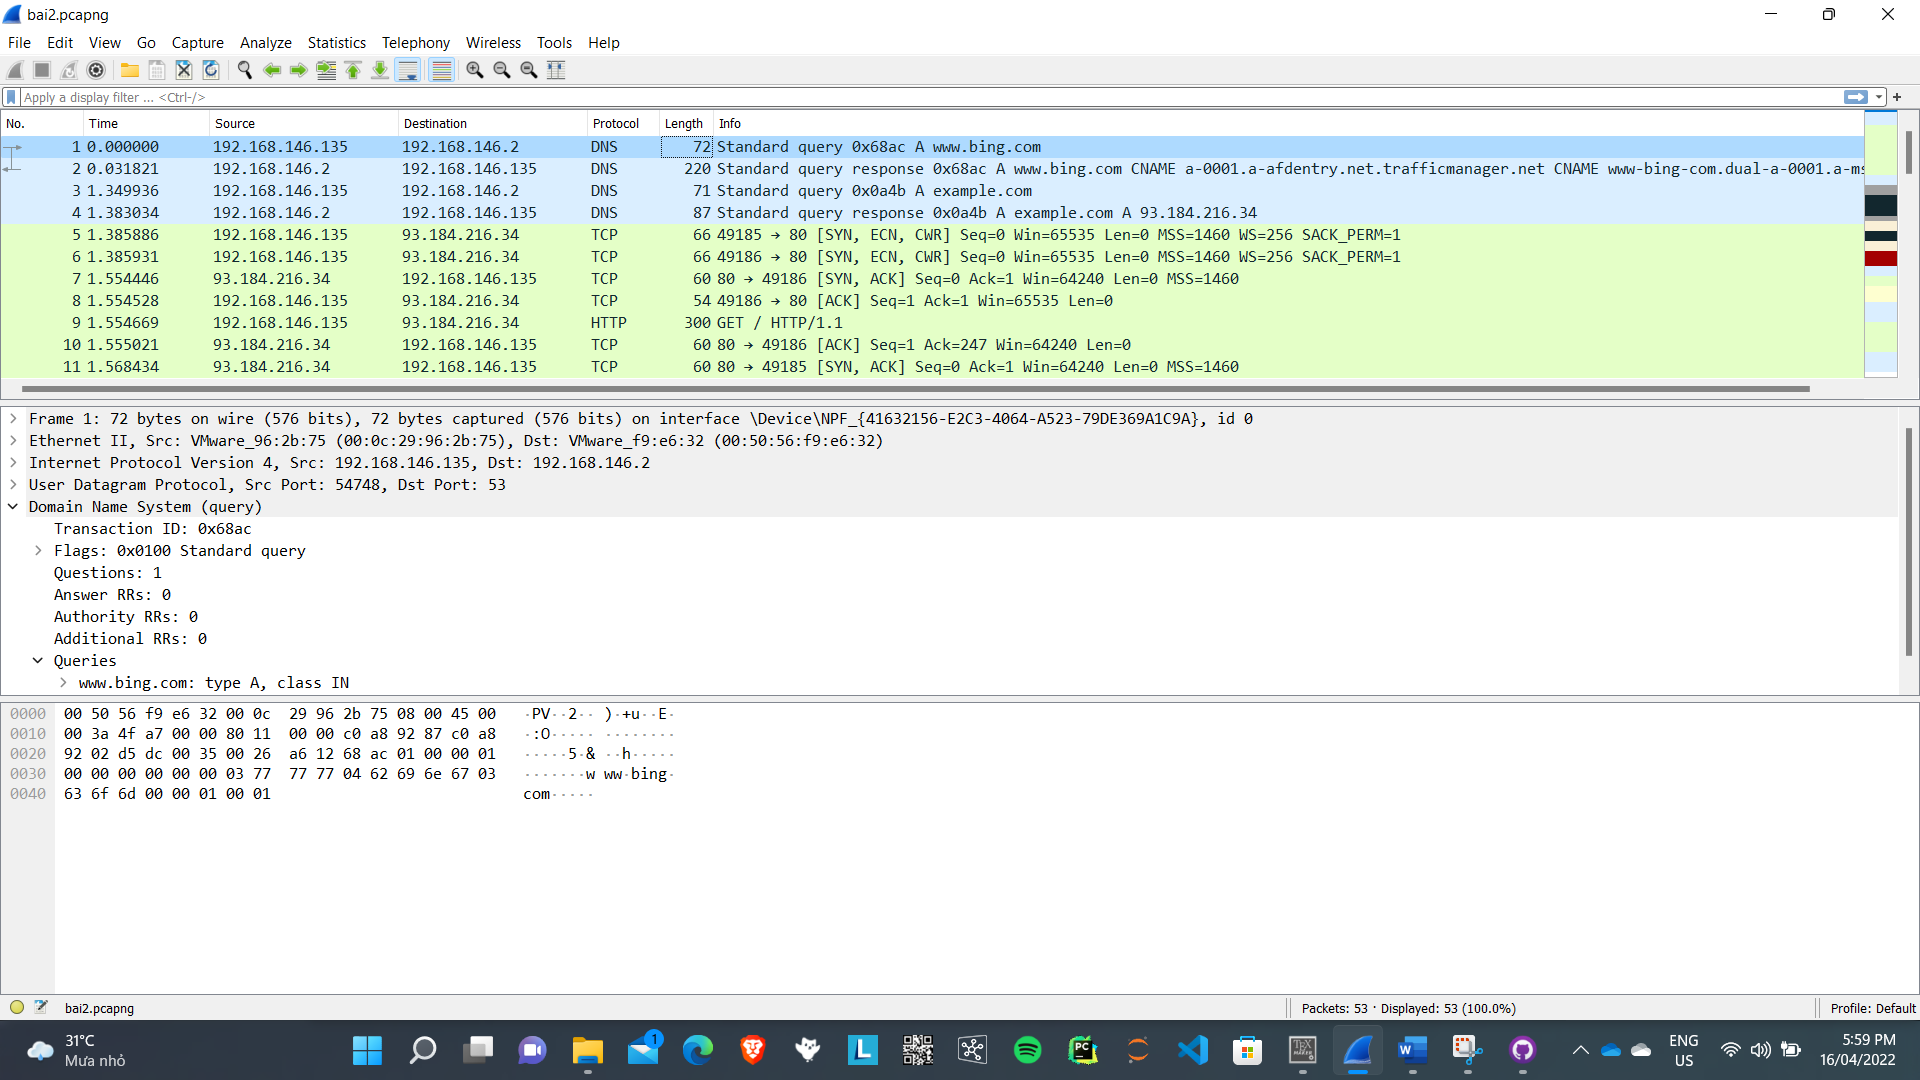
\includegraphics[scale=.45]{../figures/p2/p2_intro}
\end{center}
\caption{Kết quả bắt gói tin từ lúc bắt đầu DNS đến lúc gửi HTTP request}
\end{figure}

\textbf{2.	Cho biết IP của host.}\\
IP của host là: 93.184.216.34.
\begin{figure}[H]
\begin{center}
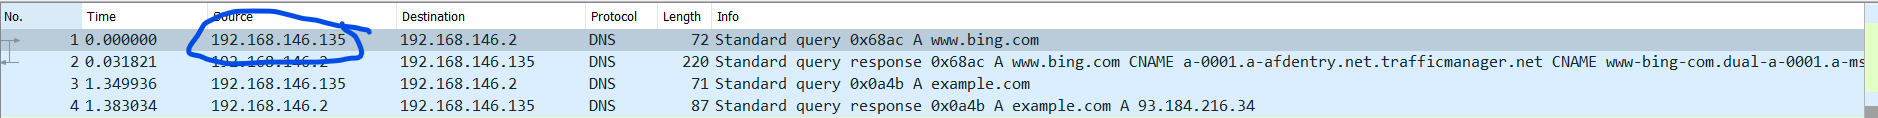
\includegraphics[scale=.6]{../figures/p2/p2_hostip}
\end{center}
\caption{IP của host}
\end{figure}

\textbf{3. Cho biết IP của router (default gateway) (nếu không thấy được thì trả lời không có và giải thích tại sao)}